% a-project.tex, v-1.0.3 marcoreis baseado no

% abntex2-modelo-trabalho-academico.tex, v-1.9.7 laurocesar
% Copyright 2012-2018 by abnTeX2 group at http://www.abntex.net.br/ 
% 
% This work consists of the files ........
% 
% -----------------------------------------------------------------------------
% Modelo para desenvolvimento de documentação de projetos acadêmicos
% (tese de doutorado, dissertação de mestrado e trabalhos de monografias em geral) 
% em conformidade com ABNT NBR 14724:2011: Informação e documentação. 
% -----------------------------------------------------------------------------
% Opções para a documentação
%
% Fancy page headings 
%\documentclass[fancyheadings, subook]{Classes/a-prj}
%\documentclass[fancyheadings, sureport]{Classes/a-prj}
%
% Fancy chapters and sections headings 
%\documentclass[fancychapter, subook]{Classes/a-prj}
%\documentclass[fancychapter, sureport]{Classes/a-prj}
%
% Fancy page , chapters and sections headings
%\documentclass[fancyheadings, fancychapter, subook]{Classes/a-prj}
\documentclass[fancyheadings, fancychapter, sureport]{Classes/a-prj}
%
% -----------------------------------------------------------------------------
% Alguns comandos para a fancy page headings)
%
% Page header line width
%\footlinewidth{value}
%
% Page footer line width
%\headlinewidth{value}
%
% Page header and footer line width
%\headingslinewidth{value}
%
% Page header and footer lines without text
%\headingslinesonly
%
% The default line width is 0.3pt.
% Set the value to 0pt to remove the page header and/or footer line
%
% -------------------------------------------------------------------------------
% Formato de figuras suportado
% -------------------------------------------------------------------------------
% O formato das figuras depende da forma como o arquivo de saída é gerado.
% As figuras inseridas na pasta Figures serão automaticamente reconhecidas sem
% a necessidade de inserir a extensão do arquivo.
%
% O pdfLaTEX (PDF) suporta figuras com as extensões: pdf, jpg, png e mps.
%
% -------------------------------------------------------------------------------
% Árvore do diretório a-project.tex
%  Diretório
%       \Classes        (requerido)
%       \Figures        (requerido) --------------------------------->
%       \Figures\PDF    (optional)
%       \Figures\JPG    (optional) Figures located within these
%       \Figures\PNG    (optional) folders are searched automatically
%       \Figures\MPS    (optional)  by the a-prj class.
%       \Figures\EPS    (optional)
%       \Figures\PS     (optional) <--------------------------------
%       \Tables         (requerido)
%       \Others         (requerido)
%       \Chapters       (requerido)
%       \Appendices     (optional)
%       \References     (requerido)
%
% -------------------------------------------------------------------------------
% PDF File resumo
\ifpdf
    \hypersetup{
    	backref,
        colorlinks  = true,
        pdftitle    = Modelo de documentação,
        pdfauthor   = {Aziel Freitas, azielfreitas@gmail.com},
        pdfsubject  = Bacharel em Engenharia,
        pdfcreator  = Subtitulo,
        pdfproducer = PDFLatex,
        pdfkeywords = {documentação, latex, dissertação, tese}}
 \fi
%
% -------------------------------------------------------------------------------
% Relação de pacotes opcionais utilizados
\usepackage[utf8]{inputenc}
\usepackage[brazil]{babel}
\usepackage{longtable}
\usepackage{dcolumn}
\usepackage{multirow}
\usepackage{lscape}
%\usepackage{graphicx}
\usepackage{rotating}
%\usepackage{float,subfigure}
%\usepackage{graphicx, subfigure}
\usepackage{cite}
\usepackage[left=3cm,top=3cm,right=2cm,bottom=2cm]{geometry}
\usepackage[alf]{abntex2cite}
\usepackage{ifpdf}
\usepackage{shadow}
\usepackage{wrapfig}
\usepackage[normalem]{ulem}
\usepackage{makeidx}
\usepackage{yfonts}
\usepackage{algorithm}
\usepackage{algorithmic}
\usepackage{lmodern}
\usepackage[T1]{fontenc}
\usepackage{indentfirst}
\usepackage{color}
\usepackage{microtype}
\usepackage{lipsum}
\usepackage{caption}
\usepackage{subcaption}
%
\makeindex 
\setlength{\LTcapwidth}{\textwidth}
%
\newtheorem{theorem}{Teorema}
\newtheorem{definition}[theorem]{Definição}
%
% -------------------------------------------------------------------------------
% Configurações do pacote backref
\renewcommand{\backrefpagesname}{Citado na(s) página(s):~}
% Texto padrão antes do número das páginas
\renewcommand{\backref}{}
% Define os textos da citação
\renewcommand*{\backrefalt}[4]{
	\ifcase #1 %
		Nenhuma citação no texto.%
	\or
		Citado na página #2.%
	\else
		Citado #1 vezes nas páginas #2.%
	\fi
}
% 
% -------------------------------------------------------------------------------
% Início do documento raiz
\begin{document}
% Definição do título da página
    \university{Centro Universitário SENAI CIMATEC}
	%\faculty{Programa de...}
	%\school{Escola de...}
% 
    %\course{Engenharia Elétrica}
    \typework{Fundamentos de Robótica Móvel}
% 
	%\course{Mestrado em Modelagem Computacional e Tecnologia Industrial}
	%\typework{Disserta\c{c}\~ao de mestrado}
	%\typework{Exame de Qualificação de Mestrado}
% 
	%\course{Engenharia Elétrica}
	%\typework{Tese de doutorado}
	%\typework{Exame de Qualificação de doutorado}
%
% -------------------------------------------------------------------------------
% Informações gerais
    \thesistitle{Relatório Final do Programa de Formação em
    Robótica e Sistemas Autônomos
    }
    \hidevolume
    \thesisvolume{Volume 1 of 1}
    \thesisauthor{Aziel Freitas}
    % \thesisauthorr{John Nash}
    % \thesisauthorrr{James Clerk Maxwell}
    % \thesisauthorrrr{Nikola Tesla}
    % \thesisauthorrrrr{Sir Isaac Newton}
    %\thesisadvisor{Prof. Marco Reis, M.Eng.}
    %\hidecoadvisor
    %\thesiscoadvisor{Marco Reis}
    \thesisdegreetitle{Bacharel em Engenharia}
    \thesismonthyear{Dezembro de 2020}
% 
    \maketitlepage
%
% ----------------------------------------------------------------------------
% Inserir Folha de rosto, Nota de estilo, folha de assinaturas, dedicatoria
    \begin{folharosto}

\begin{center}
\theauthor \\
% \theauthorr \\
% \theauthorrr \\
% \theauthorrrr \\
% \theauthorrrrr \\
\end{center}
\ \\
\ \\
\ \\
\ \\
\ \\
\begin{spacing}{2}
   \begin{center}
   {\LARGE {\bf \thetitle}}
   \end{center}
\end{spacing}
\ \\
\ \\
\ \\
\vspace*{85mm}
% \begin{flushright}

%    \begin{list}{}{
%       \setlength{\leftmargin}{7.5cm}
%       \setlength{\rightmargin}{0cm}
%       \setlength{\labelwidth}{0pt}
%       \setlength{\labelsep}{\leftmargin}}

%       \item \thetypework apresentada ao \thefaculty, Curso de \thecourse
%       do \theuniversity, como requisito parcial para a obten\c{c}\~ao do
%       t\'itulo de {\bf \thedegreetitle}.

%       \begin{list}{}{
%       \setlength{\leftmargin}{0cm}
%       \setlength{\rightmargin}{0cm}
%       \setlength{\labelwidth}{0pt}
%       \setlength{\labelsep}{\leftmargin}}

%       \item \'Area de conhecimento: Interdisciplinar

%       \item Orientador: \theadvisor
%       \newline \hspace*{2.1cm}  %{\it \theuniversity}

%       \end{list}
%    \end{list}

% \end{flushright}
\ \\
\ \\
\ \\
\ \\
%\begin{spacing}{1.5}
   \begin{center}
   Salvador \par
   \theuniversity \par
   2020
   \end{center}
%\end{spacing}

\end{folharosto}

    %\include{Others/NotaEstilo}
    %\include{Others/FolhaAssinaturas}
    %\include{Others/dedicatoria}
    %\include{Others/agradecimentos}
%
% ----------------------------------------------------------------------------
% Resumo/abstract, sumário e siglas
    \begin{romanpagenumbers}
        \begin{thesisresumo}

  Este relatório visa exibir de forma resumida os resultados dos projetos executados no curso de formação em Robótica e Sistemas Autônomos. O projeto abraçou 12 graduados nas áreas de Engenharia Elétrica, Mecânica, da Computação e de Automação e Controle e os treinou no uso de ferramentas CAD na modelagem de objetos, ferramentas de simulação, de gerenciamento de projetos, de desenvolvimento e versionamento de códigos nas linguagens Python, C++ (especialmente para ROS) e R. Essas ferramentas foram gradualmente aprendidas para que pudessem ser utilizada ao longo do programa de formação na confecção um manipulador robótico e na configuração uma plataforma móvel para realizar mapeamento e navegação autônomas, além da manipulação. Os projetos foram organizados de modo a alocar as capacidades dos graduados em equipes contendo diversidades de conhecimentos, havendo sempre a figura de um líder de projetos.

\ \\

% use de três a cinco palavras-chave

\textbf{Palavras-chave}: Robótica, Manipuladores,ROS, Linguagens de programação, Estatística

\end{thesisresumo}
        \begin{thesisabastract}
This report sums up the results of the projects executed along the duration of the graduation course in Robotics and Autonomous Systems. The
course embraced 12 graduates from the Electric, Mechanic, Computer and Control and Automation engineering fields and trained them in using CAD tools for object modelling, simulation tools for physics and environments, project management, software development in Python, C++ (specially for ROS) and R languages, as well as version management. These tools were gradually learned so that they would be used in assembling a robotic manipulator and setting up a mobile platform that was used in autonomous mapping and navigation, besides the manipulation task. The projects were fashioned so the graduates capacities would be complimentary, having present always the figure of a project leader.
\ \\

\textbf{Keywords}: Robotics, Manipulators, ROS, Programming languages, Statistics

\end{thesisabastract}

        % Make list of contents, tables and figures
        \thesiscontents
        %Include other required section
        %\include{Others/abbreviation}
        %\include{Others/simbolos}
        %Switch the page numbering back to the default format
    \end{romanpagenumbers}
%
% ---------------------------------------------------------------------------
% Include thesis chapters
    \parskip=\baselineskip
    \chapter{Introdução}
\label{chap:intro}

Este relatório traz os objetivos do programa, a sua justificativa e os conhecimentos envolvidos durante o curso de formação, além dos trabalhos realizados, materiais e métodos empregados na realização de cada projeto e o que resultou ao final de cada etapa.

%--------- NEW SECTION ----------------------
\section{Objetivos}
\label{sec:obj}

Os objetivos do programa foram: a realização dos desafios propostos, na forma de projetos e a confecção dos relatórios pertinentes, mostrando o desenvolvimento do conhecimento necessário bem como a estrutura de cada um desses projetos e seus resultados.

\subsection{Objetivos Específicos}
\label{ssec:objesp}

O relatório resume o processo de formação de um pesquisador em robótica e sistemas autônomos em treinamento pelo Laboratório de Robótica e Sistemas autônomos. Este processo contou com a ambientação em um Laboratório contendo uma estrutura física dispondo de dispositivos diversos já consolidados no mundo da robótica. Bastante consolidados também foram os diversos recursos \textit{open software} utilizados na concepção dos projetos. No curso de um ano todas essas ferramentas foram sendo utilizadas juntamente com os métodos de gerenciamento de projetos já dominados pelos Orientadores liderando o programa de formação.

%--------- NEW SECTION ----------------------
\section{Justificativa}
\label{sec:justi}

Os trabalhos desenvolvidos e certificados recebidos estão agregados neste relatório, em apêndice ao seu final, a fim esclarecer quais conhecimentos foram adquiridos ao longo do programa, bem como os métodos empregados.



%--------- NEW SECTION ----------------------
\section{Organização do documento}
\label{section:organizacao}

Este documento apresenta $5$ capítulos e está estruturado da seguinte forma:

\begin{itemize}


  \item \textbf{Capítulo \ref{chap:intro} - Introdução}: Neste capítulo estão descritos os objetivos gerais e específicos, a justificativa e como está organizado este relatório;
  \item  \item \textbf{Capítulo \ref{chap:desenvolvimento} - Desenvolvimento}: Estão descritos os projetos realizados durante o curso;
  \item \textbf{Capítulo \ref{chap:metodologia} - Metodologia}: Neste capítulo está descrita a metodologia empregada no curso de formação em Robótica e Sistemas Autônomos; 
  \item \textbf{Capítulo \ref{chap:result} - Métodos e Resultados}: Foram apresentados os métodos e os resultados obtidos nos artigos apresentados;
  \item \textbf{Capítulo \ref{chap:conc} - Conclusão}: Apresenta as conclusões em relação ao programa de formação.

\end{itemize}

    \include{Chapters/fundamentos}
    \chapter{Metodologia}
\label{chap:metodologia}

Um dos pontos característico do programa de Formação em Robótica é a sua metodologia, onde buscará a aprendizagem ativa do estudante, com a construção dos seus conhecimentos, complementando as aulas expositivas com atividades e dinâmicas de grupo, elaboração e apresentação de trabalhos e pesquisas, emprego de meios audiovisuais, estudos individualizados, pesquisa de artigos técnicos e científicos, entre outros condicionantes ao programa.
A metodologia em si é um caminho para o sucesso na formação dos estudantes, pois esta convergência baseia-se em 5 pontos principais:

\begin{enumerate}
    \item \textbf{Criatividade:} espaço que estimula a criatividade, possibilitando interação e acesso à diferentes tecnologias.
    \item \textbf{Engajamento:} atividades práticas de aprendizado aumentam os níveis de concentração
    \item \textbf{Programação:} a inteligência artificial se torna cada vez mais presente nas escolas e escritórios
    \item \textbf{Trabalho em equipe:} robótica incorpora uma gama de habilidades e promove um ambiente de aprendizagem para pessoas com diferentes talentos
    \item \textbf{Diversão:} aprender sobre robótica deve ser divertido, e a medida que os estudantes continuem melhorando sua interação com eles, isso aumenta mais ainda o nível de diversão
\end{enumerate}


Basicamente o caminho para o sucesso compreende em 4 fases distintas, demonstradas na Figura \ref{fig:metodologia}:

\textbf{Assimilação:} desenvolver habilidades de codificação e lógica;

\textbf{Simulação:} testar as missões de um robô de forma eficiente;

\textbf{Integração:} garantir informações sobre o ambiente e o robô;

\textbf{Criação:} elaborar um projeto aplicado a tecnologia.

As três primeiras fases são compreendidas em 6 meses, ficando a fase Criação com 6 meses para finalizar o programa.
Entre cada fase, desafios são lançados para que o estudante obtenha maior sucesso na assimilação dos conceitos ministrados, para a última fase um projeto final é lançado para que o estudante possa realizar a demonstração de seu sistema para os avaliadores.
Bom salientar que durante as fases, temas serão tratados e discutidos de forma expositiva e prática.


\begin{figure}[H]
    \caption{Metodologia do Programa de Formação em Robótica e Sistemas Autônomos}
    \centering
    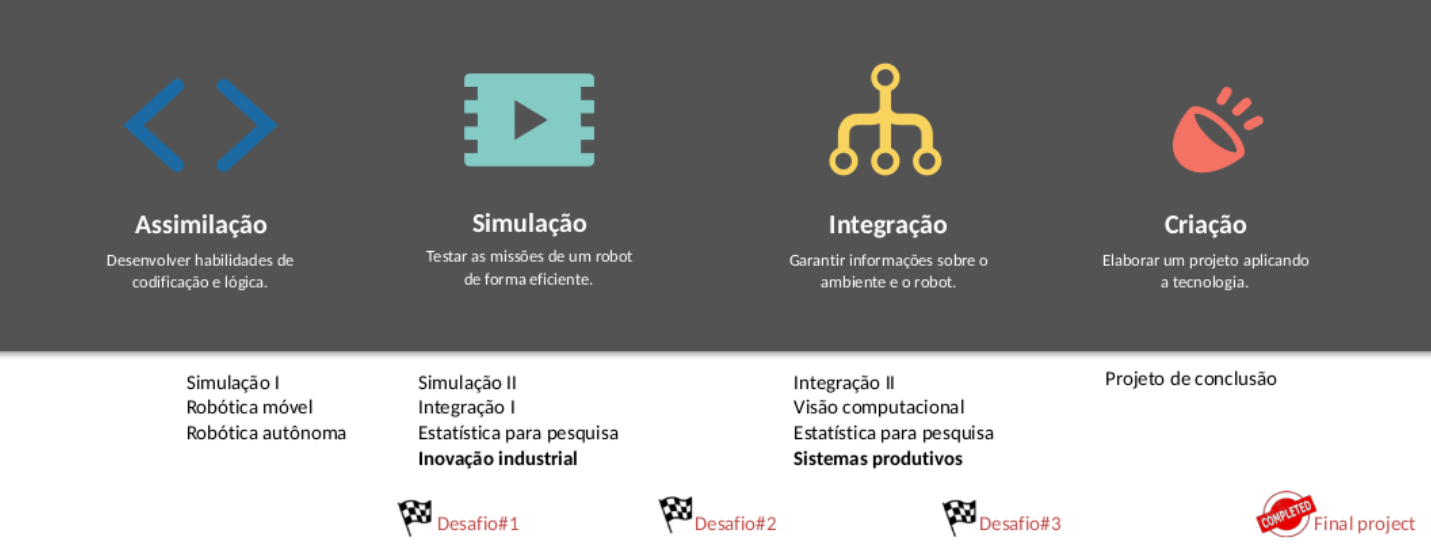
\includegraphics[width= \textwidth]{Figures/metodologia.png}
    \caption*{Fonte: Programa de Formação em Robótica e Sistemas Autônomos}
    \label{fig:metodologia}
\end{figure}

Com uma abordagem inovadora, o programa tenta realçar a busca por um aprendizado mais real e excitante para isso o conceito de professor facilitador que estimule a experiência nas várias tecnologias se faz necessário. Isso promoverá vários feedbacks mais intensos aos estudantes. Em resumo o professor será o facilitador de uma experiência de aprendizado, criando recursos e experiência para a formação do aprendiz.

% Nas próximas seções estarão descritos os materiais e métodos aplicados para cada projeto realizado durante o curso de formação em Robótica e Sistemas Autônomos. 

%\section{Desafio 1.0}
%\label{sec:met_desafio1}
%Este desafio foi feito individualmente, e ele foi realizado com o objetivo de programar o robô da \textit{Clearpath Robotics- Husky}, no ambiente de simulação do \textit{Gazebo}. A área de operação desse robô foi a área externa entre os prédios do CIMATEC 3 e 4. O \textit{Husky} tinha como missão explorar esse ambiente externo a procura de uma bola amarela, e ao identificar esta ele deveria ir até ela e parar de frente para mesma informando que a missão foi completada. Como nesse desafio foi realizada apenas a simulação, apenas o computador foi utilizado.  

%--------- NEW SECTION ----------------------
% \section{Manipulador TIMON-HM- Desafio 2.0}
% \label{sec:met_desafio2}
% O segundo desafio foi realizado em grupo, onde um manipulador deveria ser concebido desde sua fase inicial modelando toda sua estrutura e posteriormente realizada a simulação deste no \textit{Gazebo}, com a missão da câmera integrada ao manipulador identificar o \textit{tag ArUco} na caixa e pressionar o botão. Este desafio também foi realizada apenas a simulação, por isso apenas o computador foi utilizado.  

% %--------- NEW SECTION ----------------------
% \section{Manipulador Robótico JeRoTIMON- Desafio 2.2 }
% \label{sec:met_desafio2_2}
% Este desafio foi para construir o modelo real do manipulador JeRoTIMON modelado e simulado no desafio \ref{sec:met_desafio2}, realizado em grupo, onde o objetivo era o mesmo, reconhecer a \textit{tag ArUco} na caixa e pressionar o botão, só que dessa vez no ambiente real. Os materiais utilizados nesse desafio foram perfis de alumínio, motores \textit{Dynamixel}, câmera RGB modelo \textit{Teledyne Genie Nano C2590},  peças modeladas no \textit{OnShape} e impressas em \textit{ABS} por uma impressora 3D, conexões para alimentação e para comunicação

% %--------- NEW SECTION ----------------------
% \section{TIMON- HM- Desafio 2.5}
% \label{sec:met_desafio2_5}
% O desafio 2.5 foi realizado em equipe, a mesma do desafio \ref{sec:met_desafio2}, onde o robô programado foi o \textit{Darwin-OP} e este deveria realizar duas missões, a primeira, é a marcha, onde quatro robôs \textit{Darwin-OP} deveriam andar de forma sincronizada de um ponto a outro da pista de corrida. E a segunda missão foi realizada a programação para que os quatro robôs realizassem a corrida com revezamento, onde cada robô está posicionado numa parte específica da pista de corrida e ao chegar próximo um do outro eles mantém por um período a movimentação sincronizada depois o anterior para e o outro segue, igualmente a uma corrida com revezamento real.


% %--------- NEW SECTION ----------------------
% \section{UGV SACI: Integrado com Detecção Visual e Manipulador- Desafio 3.0}
% \label{sec:met_desafio3}
% Neste desafio foi desenvolvido o Saci, que integra o veículo autônomo da \textit{Clearpath Robotics Warthog} equipado com sensores (câmeras, LiDAR e GPS) e o manipulador robótico JeRoTIMON, com o propósito de transformá-lo em um robô autônomo. Este foi construído com o intuito de que o mesmo tivesse navegação autônoma para realizar investigação em ambiente externo e construir um mapa deste ambiente, detectasse a "bomba" escondida, e realizasse o desarme da bomba através do manipulador. 
% Esse projeto foi desenvolvido em duas etapas, a de simulação, onde foram utilizados o software  \textit{Gazebo} e a ferramenta de visualização \textit{Rviz}, e para configuração do pacote de parâmetros do manipulador foi utilizado \textit{MoveIt}. E em paralelo foi desenvolvido este robô em sua versão real, onde foi possível realizar testes e verificar seu desempenho em campo.



% \section{Analíse estatística R\&R da simulação do robô Darwin OP}
% \label{sec:met_analise_darwin}
% Teve como objetivo analisar o sistema de medição dos dados coletados durante os testes realizados nas etapas: de marcha e de revezamento do Desafio 2.5 (\ref{sec:met_desafio2_5}), utilizando o método de análise de variância (ANOVA). Nessa análise foi possível aplicar os conhecimentos obtidos em estatística, utilizando a ferramenta e linguagem de programação \textit{R} em um projeto realizado durante o curso, a fim de verificar o desempenho desse projeto, exemplo, a análise de precisão produzida através do estudo R\&R (Repetibilidade e Reprodutibilidade). Foram utilizadas apenas as ferramentas de simulação e para realização do estudo estatístico.


% \section{Planejamento de Experimentos (DOE) -Helicóptero de Papel (TIMON-HM)}
% \label{sec:met_analise_doe}
% Esse experimento teve como objetivo aplicar os conceitos de Planejamento de Experimento- \textit{DOE}, a um modelo de helicóptero de papel. O propósito principal foi identificar quais são os fatores que mais influenciam seu tempo de voo e como estas variáveis podem melhorar o seu desempenho. Durante o processo, foi utilizado um modelo de helicóptero em papel onde foi medido o seu tempo de voo em duas alturas diferentes, além disto, foram adicionados adesivos e um clipe em sua estrutura a fim de verificar a influência da variação destes parâmetros no resultado final. Esse estudo proporcionou a aplicação do aprendizado adquirido ao uso da ferramenta e linguagem R usada para manipulação, análise e visualização de dados, e dos conhecimentos de Estatística. 

% \section{Artigo publicado TRIS: Thermal Remote Identification System of Feverish People }
% \label{sec:met_tris}

% Esse artigo, que possui também um sistema real de mesmo nome \textit{(TRIS)}, foi modelado a partir da necessidade exposta pela pandemia do COVID-19, para identificar pessoas  foram usadas câmeras (RGB e Infravermelho), um computador para utilizar uma rede neural, e que identificasse pessoas com temperatura acima de 37,8 $^\circ$C, e informasse que aquela pessoa em questão era objeto de interesse pois estaria com febre, ou estado febril, que é um dos sintomas do COVID-19. Esse sistema foi criado com o próposito de realizar o controle da propagação do vírus. Nesse projeto puderam ser desenvolvidos os conhecimentos de rede neural, interface de sistemas, utilização de câmeras RGB e Infravermelho, e a como acontece a evolução de um projeto.
    \chapter{Resultados}
\label{chap:result}

Nesta seção serão demonstrados os métodos e resultados dos artigos provenientes dos
trabalhos desenvolvidos durante o período do curso de formação em Robótica e Sistemas Autônomos. Nos Apêndices estão identificados os artigos publicados e certificados obtidos.

%--------- NEW SECTION ----------------------
\section{Artigo SAPCT}
\label{sec:artigoRAJA}

Para o evento V Seminário de Avaliação de Pesquisa Científica e Tecnológica (SAPCT)
foi realizado o artigo Projeto e Simulação de um Manipulador Robótico com 5 Graus de
Liberdade e Sistema de Visão Integrado, com base no projeto do manipulador robótico
RAJA, este artigo consta no Apêndice \ref{app:rajapaper}. O trabalho apresentado foi premiado como melhor trabalho na categoria de bolsistas de projeto PD\&I.


\section{Integração do sistema}
\label{sec:artigoTRIS}

Esse artigo refere-se ao projeto ``TRIS'' que foi criado a partir da necessidade gerada pela pandemia do COVID-19 de isolar possíveis vetores do vírus. Seu funcionamento é dado pela identificação de pessoas e avaliação das suas temperaturas através de câmeras (RGB e espectro infravermelho). Os algoritmos requerem um computador treinado através de uma rede neural no reconhecimento de rostos e aferição da temperatura. Caso valores acima de 37,8$\circ$C sejam detectados, o programa irá alertar um operador diante do sistema para que este informasse à pessoa sobre a possibilidade dela estar num ou estado febril, que é um dos sintomas do COVID-19. Esse sistema foi criado com o próposito de auxiliar no controle da propagação do vírus. Nesse projeto puderam ser desenvolvidos os conhecimentos de rede neural, interface de sistemas, concepção de um banco de dados, utilização de câmeras RGB e espectro infravermelho. O resultado obtido do projeto do TRIS foi o artigo publicado no evento VI International Symposium on Innovation and Technology (SIINTEC) 2020, e posteriormente sua premiação em primeiro lugar dentre os trabalhos apresentados. Este artigo e o certificado de participação nestes evento constam, respectivamente, nos Apêndices \ref{app:trispaper} e \ref{app:certif}




    \chapter{Conclusão}
\label{chap:conc}

A especialização em Robótica e Sistemas autônomos proporcionada pelo Laboratório de Robótica e Sistemas Autônomos do SENAI CIMATEC extensa e abrangente, uma convergência de métodos, técnicas e conhecimentos de diversas áreas, como naturalmente acontece em pesquisas em Robótica, um campo de incontáveis possibilidades. O Laboratório é fruto dos esforços de pesquisadores já experientes, e a sua intenção de capacitar futuros companheiros de trabalho foi o que gerou o programa de capacitação ``Novos Talentos'', o qual fiz parte juntamente com outros 11 colegas.

As diversas etapas presentes na condução de projetos de pesquisa em Robótica foram trazidas nas formas dos Desafios propostos nas seções expostas no Capítulo \ref{chap:desenvolvimento}, e analisar estes documentos revela a amplitude de tarefas e conhecimento necessários para o sucesso em um projeto. Não tão transparente, todavia, está o aparato e os métodos utilizados em gerência de projetos. Este tema foi amplamente explorado embora uma documentação expressiva não tenha sido gerada. 

    % include more chapters ...
%
% ----------------------------------------------------------------------------
% Include thesis appendices
    \begin{thesisappendices}
        \include{Appendices/diagmec}
        \include{Appendices/diagele}
        \include{Appendices/logbook}
    \end{thesisappendices}
%
% ----------------------------------------------------------------------------
% Configurar as referencias bibliograficas
	\renewcommand\bibname{Referências}
    \addcontentsline{toc}{chapter}{Referências}
    \bibliography{References/referencias}
%
% ----------------------------------------------------------------------------
% Finishing him
    \include{Others/ultimafolha}
\end{document}
%
% -------------------------------------------------------------------------------
% Aqui termina a formatação para o documento.
% In God We Trust. All Other Bring Data. 
%
% -------------------------------------------------------------------------------